% Para cuando se tenga la carta firmada, scaneada y en formato PDF
% 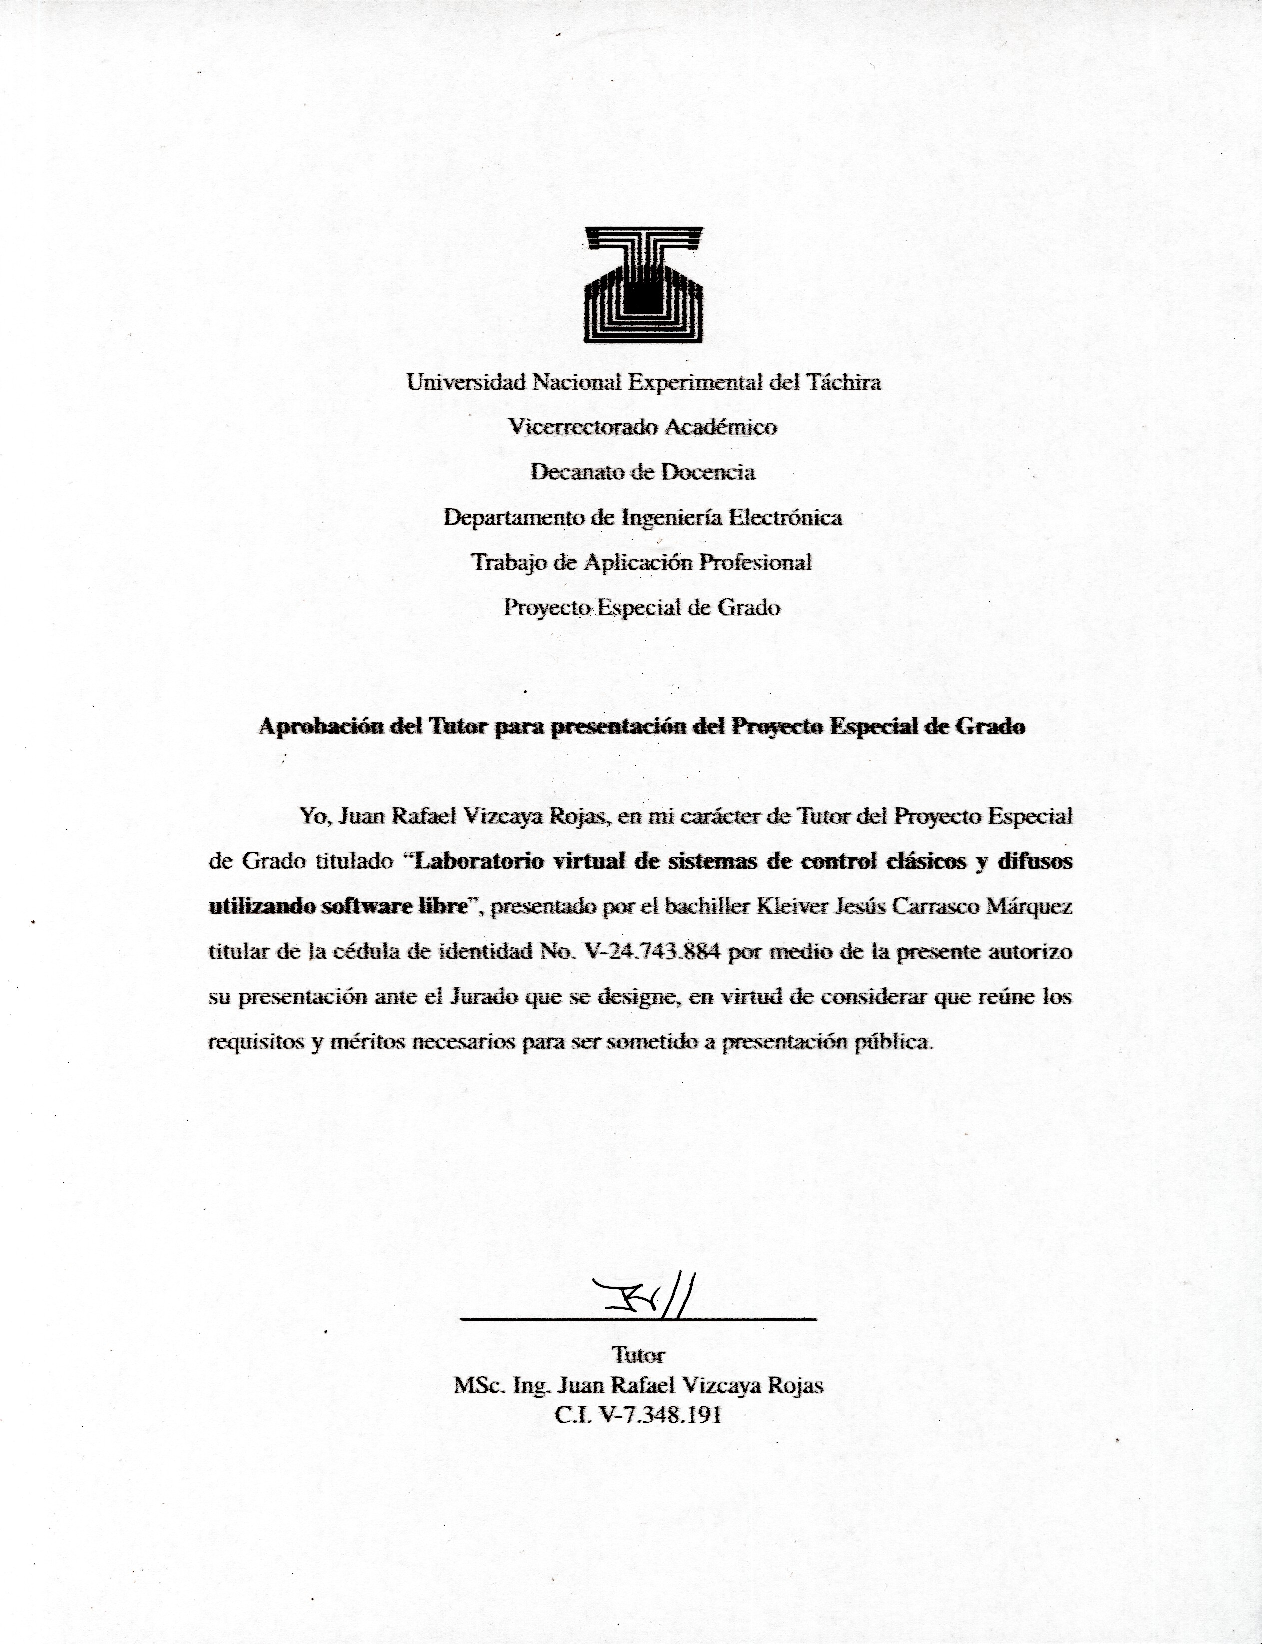
\includepdf[pages=-, fitpaper,
% 				templatesize={\paperwidth}{\paperheight},
% 				pagecommand={\thispagestyle{empty}\setcounter{page}{3}}
%                 ]{FrontContent/cartaAprobacion}

% Generación de la carta
\begin{titlepage}
\parskip=7.25pt plus 2pt
\setcounter{page}{3}
\begin{center}
    \begin{spacing}{1}
    % Logo de la unet --------------------------------------------
    
\includegraphics[width=2cm]{unet.jpg}
    
    Universidad Nacional Experimental del Táchira 
    
    Vicerrectorado Académico
    
    Decanato de Docencia
    
    Departamento de Ingeniería Electrónica
    
    Trabajo de Aplicación Profesional
    
    Proyecto Especial de Grado
    \end{spacing}
\end{center}

\vspace{0.5cm}

\begin{center}
        
        \textbf{Aprobación del Tutor para presentación del Proyecto Especial de Grado}
        
\end{center}

\vspace{0.5cm}

\begin{spacing}{1.5}
    Yo, Juan Rafael Vizcaya Rojas, en mi carácter de Tutor del Proyecto Especial de Grado titulado \enquote{\textbf{Laboratorio virtual de sistemas de control clásicos y difusos utilizando software libre}}, presentado por el bachiller Kleiver Jesús Carrasco Márquez titular de la cédula de identidad No. \mbox{V-24.743.884} por medio de la presente autorizo su presentación ante el Jurado que se designe, en virtud de considerar que reúne los requisitos y méritos necesarios para ser sometido a presentación pública.
\end{spacing}

\vfill

\begin{center}
    
    \rule{6cm}{1pt}
    
    \vspace{0.2cm}
    
    \parskip=0pt plus 2pt
    
    \begin{spacing}{1}
        Tutor
    
        Juan Rafael Vizcaya Rojas
    
        C.I. V-7.348.191
    \end{spacing}
    
\end{center}

\vspace{0.5cm}

\end{titlepage}
